Jeder Agent hält eine individuelle Entfernungskarte. Die grundlegende Aufgabe dieser Karte ist es, die Entfernung zum Ziel des Agenten wiederzugeben. Sie ist als Tabelle zu verstehen, in der für jede Zelle notiert ist, wie viele Bewegungsschritte nötig wären, um das Ziel von dieser Zelle aus zu erreichen. Diese Entfernungen werden durch eine einfache Breitensuche ermittelt. Die aktuelle Position des Agenten ist dabei nicht interessant. Der CoDy Algorithmus ist auch in der Lage mit unbekannten Umgebungen umzugehen. \cite{book:regele} \newline Zum einen ist das für den Anwendungsfall in erster Linie nicht interessant und zum anderen würde dies die Komplexität unnötig erweitern. Deshalb ist eine Entfernungskarte, im Kontext dieser Arbeit, eine Karte, die die gesamte Umgebung erfasst.
\begin{figure}[H]
    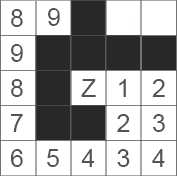
\includegraphics[height=40mm]{images/example_distancemap.png}
    \centering
    \caption{Beispiel für eine kleine Entfernungskarte}
    \label{fig:example_distancemap}
\end{figure}
Abbildung \ref{fig:example_distancemap} zeigt beispielhaft eine Entfernungskarte. Die grauen Zellen stellen statische Hindernisse dar. Das "'Z"' ist das Ziel des Agenten. Die Zahlen sind die Entfernungen und weiße Zellen sind nicht erreichbar.